As the dataset had a lot of \verb|null| columns and cells, first resolved that issue by dropping the \textbf{null} columns.
After then moved on the \verb|null/NaN| cell and took care of it as well by dropping the null/NaN rows.
Did the necessary encoding(binary label encoding where 0 means non-spam and 1 means spam) for the label and got rid of duplicates values from rows.
After performing these series of data-preprocessing steps, I ended up with \textbf{5693} rows and \textbf{2} columns.
However, converting the plain raw email texts into features was yet to be done.
To achieve this, I used two slightly different text \verb|vectorizer/tokenizer|\textit{(count the frequency of words in texts ignoring some common stop words that have no significant impact on the meaning of the sentences but appear frequently)}\cite{countvectorizer_in_nlp_2020}
namely \verb|CountVectorizer()| and \verb|TfidfVectorizer()| to convert them into features so that later I can train and test various models on them.
After preprocessing the dataset, the dataset contained around \textbf{37000}) features or words\textit{(tokens)} found by \verb|CountVectorizer()| and \verb|TfidfVectorizer()|.
To get an idea about each set of features, I used \verb|wordcloud| to generate visual representations of the most frequently occurring words shown in the below Figure~\ref{fig:cout_vect} and Figure ~\ref{fig:tfidf_vect}.

\begin{figure}[H]
    \begin{center}
        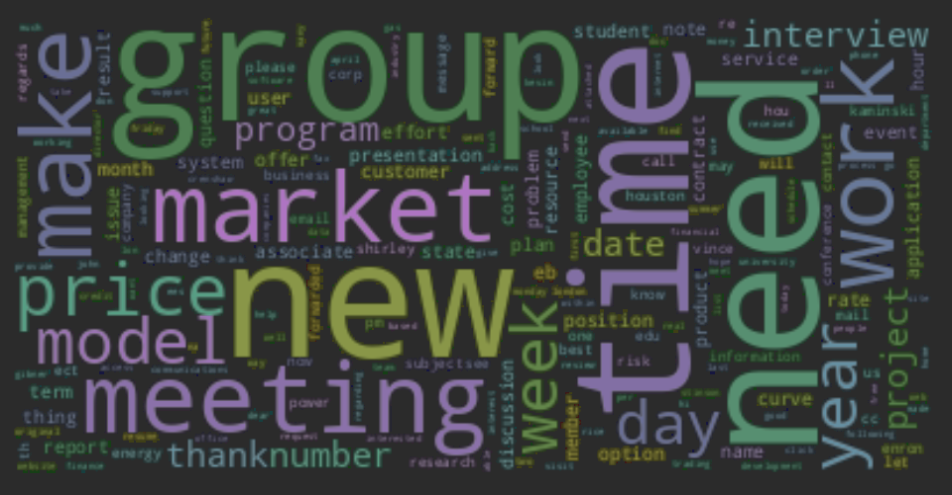
\includegraphics[scale=0.4]{Graphics/images/count_vect}
    \end{center}
    \caption{Frequent Words Found Using count vectorizer}
    \label{fig:cout_vect}
\end{figure}

\begin{figure}[H]
    \begin{center}
        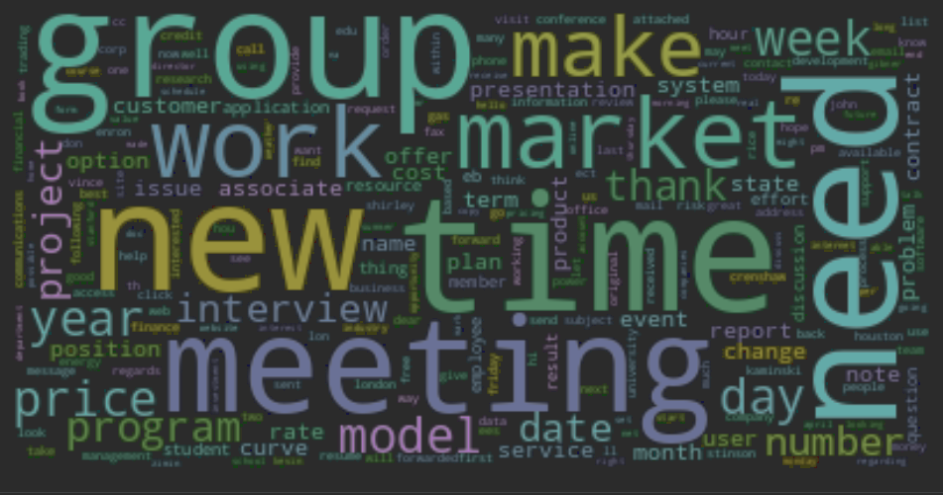
\includegraphics[scale=0.4]{Graphics/images/tfid_vect}
    \end{center}
    \caption{Frequent Words Found Using tfidf vectorizer}
    \label{fig:tfidf_vect}
\end{figure}